%=======================================================================
\section{Results \& Visualization}
%=======================================================================

\subsection{Stage A: chosen sets}

\begin{table}[H]
\centering
\caption{Chosen sets. Absolute values are listed as KDDCup99 / Covertype / INSECTS.}
\label{tab:sets}
\footnotesize
\begin{tabularx}{\textwidth}{@{}l l L@{}}
\toprule
\textbf{Algorithm} & \textbf{Method} & \textbf{Chosen set} \\
\midrule
DenStream & Default       & $\varepsilon=0.02$, $\beta=0.75$, $\mu=2$ \\
          & Arm 1 = Arm 2 & $\varepsilon=5.5$, $\beta=0.2$, $\mu=20$ \\
          & Arm 3         & $\varepsilon=1.6\cdot s(D) = 1360 / 3668 / 5221$, $\beta=0.5$, $\mu=5$ \\
          & P2R           & $\varepsilon = 680 / 459 / 1305$, $\beta=0.5$, $\mu=5$ \\
\midrule
CluStream & Default       & $k=5$, $q=100$, $t=2$ \\
          & Arm 1 = Arm 2 & $k=8$, $q=50$, $t=2$ \\
          & Arm 3         & $k=8$, $q=16$, $t=2$ \\
          & P2R           & $k=4/8/16$, $q=8/16/32$, $t=2$ \\
\bottomrule
\end{tabularx}
\end{table}

\begin{table}[H]
\centering
\caption{Stage A ARI, 50k samples, averaged over 5 datasets.}
\label{tab:phaseA}
\small
\begin{tabular}{@{}l l c c c@{}}
\toprule
\textbf{Algorithm} & \textbf{Method} & \textbf{In-sample} & \textbf{LODO} & \textbf{Optimism} \\
\midrule
DenStream & Default & 0.044 & --    & --    \\
          & Arm 2   & 0.073 & 0.044 & 0.029 \\
          & Arm 3   & 0.113 & 0.079 & 0.034 \\
          & P2R     & 0.110 & \textbf{0.109} & \textbf{0.001} \\
\midrule
CluStream & all methods & $\le 0.005$ & $\le 0.004$ & -- \\
\bottomrule
\end{tabular}
\end{table}
\takeaway{For DenStream, relative parameters help: Arm 3 beats Arm 2 by $0.035$ on LODO. P2R loses almost nothing on unseen datasets because it re-reads the granularity on each one.}

\subsection{Stage B: full-length runs}

\pgfplotsset{
  arifig/.style={
    ybar, bar width=5pt, width=0.52\linewidth, height=5cm,
    symbolic x coords={KDD,Cov,INS}, xtick=data,
    xticklabels={KDDCup99, Covertype, INSECTS},
    tick label style={font=\scriptsize}, label style={font=\scriptsize},
    title style={font=\small}, ylabel={ARI},
    ymajorgrids, grid style={gray!25}, enlarge x limits=0.22,
    extra y ticks={0}, extra y tick style={grid=major, grid style={black}},
    scaled y ticks=false, yticklabel style={/pgf/number format/fixed},
  },
}
\begin{figure}[H]
\centering
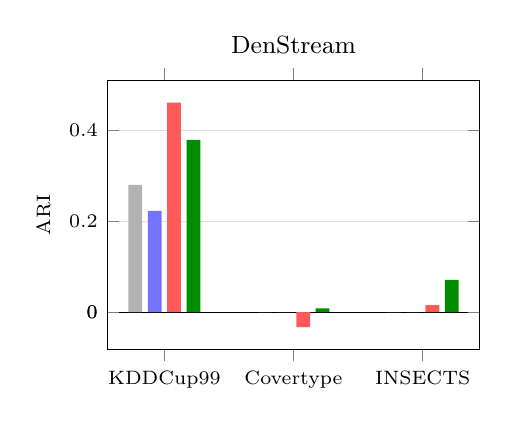
\begin{tikzpicture}
\begin{axis}[arifig, title={DenStream}, legend to name=arileg,
  legend columns=4, legend style={font=\scriptsize, draw=none}]
\addplot[fill=gray!60, draw=none]     coordinates {(KDD,0.280) (Cov,0.000) (INS,0.000)};
\addplot[fill=blue!55, draw=none]     coordinates {(KDD,0.223) (Cov,0.000) (INS,0.000)};
\addplot[fill=red!65, draw=none]      coordinates {(KDD,0.461) (Cov,-0.033) (INS,0.015)};
\addplot[fill=green!55!black, draw=none] coordinates {(KDD,0.379) (Cov,0.008) (INS,0.071)};
\legend{Default, Arm 1 = Arm 2, Arm 3, P2R}
\end{axis}
\end{tikzpicture}\hfill
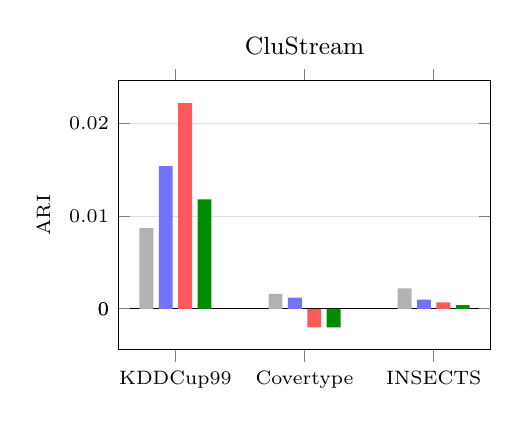
\begin{tikzpicture}
\begin{axis}[arifig, title={CluStream}]
\addplot[fill=gray!60, draw=none]     coordinates {(KDD,0.0087) (Cov,0.0016) (INS,0.0022)};
\addplot[fill=blue!55, draw=none]     coordinates {(KDD,0.0154) (Cov,0.0012) (INS,0.0010)};
\addplot[fill=red!65, draw=none]      coordinates {(KDD,0.0222) (Cov,-0.0020) (INS,0.0007)};
\addplot[fill=green!55!black, draw=none] coordinates {(KDD,0.0118) (Cov,-0.0020) (INS,0.0004)};
\end{axis}
\end{tikzpicture}

\ref{arileg}
\caption{Full-stream ARI, mean of seeds 2 and 3. The two panels use different y scales.}
\label{fig:ari}
\end{figure}

\begin{table}[H]
\centering
\caption{DenStream on full-length datasets.}
\label{tab:den_full}
\footnotesize
\begin{tabular}{@{}l ccc ccc@{}}
\toprule
& \multicolumn{3}{c}{\textbf{ARI}} & \multicolumn{3}{c}{\textbf{Throughput (samples/s)}} \\
\cmidrule(lr){2-4}\cmidrule(l){5-7}
\textbf{Method} & KDD & Cov & INS & KDD & Cov & INS \\
\midrule
Default       & 0.280 & 0.000 & 0.000 & 9{,}926 & 71{,}323 & 29{,}880 \\
Arm 1 = Arm 2 & 0.223 & 0.000 & 0.000 & 6{,}391 & 70{,}119 & 30{,}407 \\
Arm 3         & \textbf{0.461} & $-0.033$ & 0.015 & 6{,}778 & 25{,}479 & 27{,}148 \\
P2R           & 0.379 & \textbf{0.008} & \textbf{0.071} & 3{,}952 & 328 & 384 \\
\bottomrule
\end{tabular}
\end{table}
\takeaway{The default and Arms 1--2 collapse to one cluster on Covertype and INSECTS because $\varepsilon$ is far too small for their scale. Arm 3 is best on KDDCup99 but negative on Covertype. P2R is the only method that beats the default everywhere, at the cost of many more micro-clusters and much lower throughput. For CluStream, all differences are within seed noise; tuned sets only run 3--14$\times$ faster.}
